\documentclass[../main.tex]{subfiles}
\graphicspath{{\subfix{../Images/}}}

\begin{document}

\chapter{Parameters, Textures, and Expressions}

This chapter continues to present Cg concepts through a series of simple vertex and fragment programs. The chapter has the following three sections:

\FloatBarrier
\begin{itemize}
\item \textbf{"Parameters"} explains how Cg programs handle parameters.
\item \textbf{"Texture Samplers"} explains how fragment programs access textures.
\item \textbf{"Math Expressions"} shows how math expressions compute new vertex and fragment values.
\end{itemize}

\section{3.1 Parameters}

The \textbf{C2E1v_green} and \textbf{C2E2f_passthrough} examples from Chapter 2 are very basic. We will now broaden these examples to introduce additional parameters.

\subsection{3.1.1 Uniform Parameters}

\textbf{C2E1v_green} (see page 38 in Chapter 2) always assigns green for the vertex color. If you rename the \textbf{C2E1v_green} program and change the line that assigns the value of \textbf{OUT.color}, you can potentially make a different vertex program for any color you like.

For example, changing the appropriate line results in a hot pink shader:

\FloatBarrier
\begin{lstlisting}
  OUT.color = float4(1.0, 0.41, 0.70, 1.0); // RGBA hot pink
\end{lstlisting}
\FloatBarrier

The world is a colorful place, so you wouldn't want to have to write a different Cg program for every color under the sun. Instead, you can generalize the program by passing it a parameter that indicates the currently requested color.

The \textbf{C3E1v_anyColor} vertex program in Example 3-1 provides a \textbf{constantColor} parameter that your application can assign to any color, rather than just a particular constant color.

\FloatBarrier
\begin{lstlisting}[caption=Example 3-1. The \textbf{C3E1v_anyColor} Vertex Program]
struct C3E1v_Output {
  float4 position : POSITION;
  float4 color    : COLOR;
};

C3E1v_Output C3E1v_anyColor(float2 position : POSITION,
                            uniform float4 constantColor)
{
  C3E1v_Output OUT;

  OUT.position = float4(position, 0, 1);
  OUT.color = constantColor;  // Some RGBA color

  return OUT;
}
\end{lstlisting}
\FloatBarrier

The difference between \textbf{C3E1v_anyColor} and \textbf{C2E1v_green} is the function interface definition and what each program assigns to \textbf{OUT.color}.

The updated function definition is this:

\FloatBarrier
\begin{lstlisting}
C3E1v_Output C3E1v_anyColor(float2 position : POSITION,
                            uniform float4 constantColor)
\end{lstlisting}
\FloatBarrier

In addition to the position parameter, the new function definition has a parameter named \textbf{constantColor} that the program defines as type \textbf{uniform float4}. As we discussed earlier, the \textbf{float4} type is a vector of four floating-point values—in this case, assumed to be an RGBA color. What we have not discussed is the \textbf{uniform} type qualifier.

\subsection*{The uniform Type Qualifier}

The \textbf{uniform} qualifier indicates the source of a variable's initial value. When a Cg program declares a variable as \textbf{uniform}, it conveys that the variable's initial value comes from an environment that is external to the specified Cg program. This external environment contains your 3D programming interface state and other name/value pairs established through the Cg runtime.

In the case of the \textbf{constantColor} variable in the \textbf{C3E1v_anyColor} example, the Cg compiler generates a vertex program that retrieves the variable's initial value from a vertex processor constant register within the GPU.

Using the Cg runtime, your 3D application can query a parameter handle for a uniform parameter name within a Cg program—in this case, \textbf{constantColor} —and use the handle to load the proper value for the particular uniform variable into the GPU. The details of how uniform parameter values are specified and loaded vary by profile, but the Cg runtime makes this process easy. Appendix B explains how to do this.

Our \textbf{C3E1v_anyColor} vertex program assigns the vertex output color to the value of its \textbf{constantColor} uniform variable, as shown:

\FloatBarrier
\begin{lstlisting}
  OUT.color = constantColor;  // Some RGBA color
\end{lstlisting}
\FloatBarrier

Whatever color the application specifies for the \textbf{constantColor} uniform variable is the color that the Cg program assigns to the output vertex color when \textbf{C3E1v_anyColor} transforms a vertex.

The addition of a uniform parameter lets us generalize our initial example to render any color, when originally it could render only green.

\subsection*{When There Is No uniform Qualifier}

When a Cg program does not include the \textbf{uniform} qualifier to specify a variable, you can assign the initial value for the variable in one of the following ways:

\FloatBarrier
\begin{itemize}
\item Using an explicit initial assignment:
\FloatBarrier
\begin{lstlisting}
         float4 green = float4 (0, 1, 0, 1);
\end{lstlisting}
\FloatBarrier

\item Using a semantic:
\FloatBarrier
\begin{lstlisting}
         float4 position : POSITION;
\end{lstlisting}
\FloatBarrier

\item Leaving it undefined or equal to zero, depending on the profile:
\FloatBarrier
\begin{lstlisting}
         float whatever;  // May be initially undefined or zero
\end{lstlisting}
\FloatBarrier
\end{itemize}
\FloatBarrier

\subsection*{What \textbf{uniform} Means in RenderMan vs. Cg}

\subsection*{Caution}

The \textbf{uniform} reserved word will be familiar to programmers who have written shaders in RenderMan. However, the meaning of \textbf{uniform} in Cg is different from its meaning in RenderMan.
\hrule

In RenderMan, the \textbf{uniform} storage modifier indicates variables whose values are constant over a shaded surface, whereas \textbf{varying} variables are those whose values can vary over the surface.

Cg does not have this same distinction. In Cg, a \textbf{uniform}-qualified variable obtains its initial value from an external environment and, except for this initialization difference, is the same as any other variable. Cg permits all variables to vary, unless the variable has the \textbf{const} type qualifier specified. Unlike RenderMan, Cg has no \textbf{varying} reserved word.

Despite the semantic difference between RenderMan's concept of \textbf{uniform} and Cg's concept of it, variables declared \textbf{uniform} in RenderMan correspond to variables declared \textbf{uniform} in Cg, and vice versa.

\subsection{3.1.2 The \textbf{const} Type Qualifier}

Cg also provides the \textbf{const} qualifier. The \textbf{const} qualifier affects variables the same way that the \textbf{const} qualifier does in C and C++: it restricts how a variable in your program may be used. You cannot assign a value to, or otherwise change, a variable that is specified as constant. Use the \textbf{const} qualifier to indicate that a certain value should never change. The Cg compiler will generate an error if it detects usage that would modify a variable declared as \textbf{const}.

Here are some examples of usage not allowed when a program qualifies a variable with \textbf{const}:

\FloatBarrier
\begin{lstlisting}
const float pi = 3.14159;
pi = 0.4;        // An error because pi is specified const
float a = pi++;  // Implicit modification is also an error
\end{lstlisting}
\FloatBarrier

The \textbf{const} and \textbf{uniform} type qualifiers are independent, so a variable can be specified using \textbf{const} or \textbf{uniform}, both \textbf{const} and \textbf{uniform}, or neither.

\subsection{3.1.3 Varying Parameters}

You have already seen examples of a per-vertex varying parameter in both \textbf{C2E1v_green} and \textbf{C3E1v_anyColor} . The \textbf{POSITION} input semantic that follows the \textbf{position} parameter in \textbf{C2E1v_green} and \textbf{C3E1v_anyColor} indicates that the GPU is to initialize each respective \textbf{position} parameter with the input position of each vertex processed by each respective program.

Semantics provide a way to initialize Cg program parameters with values that vary either from vertex to vertex (in vertex programs) or fragment to fragment (in fragment programs).

A slight modification to \textbf{C3E1v_anyColor}, called \textbf{C3E2v_varying}, in Example 3-2, lets the program output not merely a single constant color, but rather a color and texture coordinate set (used for accessing textures) that can vary per vertex.

\FloatBarrier
\begin{lstlisting}[caption=Example 3-2. The C3E2v_varying Vertex Program]
struct C3E2v_Output {
  float4 position : POSITION;
  float4 color    : COLOR;
  float2 texCoord : TEXCOORD0;
};

C3E2v_Output C3E2v_varying(float2 position : POSITION,
                           float4 color    : COLOR,
                           float2 texCoord : TEXCOORD0)
{
  C3E2v_Output OUT;

  OUT.position = float4(position, 0, 1);
  OUT.color    = color;
  OUT.texCoord = texCoord;

  return OUT;
}
\end{lstlisting}
\FloatBarrier

The \textbf{C3E2v_varying} example prototypes its vertex program as:

\FloatBarrier
\begin{lstlisting}
C3E2v_Output C3E2v_varying(float2 position : POSITION,
                           float4 color    : COLOR,
                           float2 texCoord : TEXCOORD0)
\end{lstlisting}
\FloatBarrier

The \textbf{C3E2v_varying} example replaces the \textbf{constantColor} parameter declared as a uniform parameter in the \textbf{C3E1v_anyColor} example with two new nonuniform parameters, \textbf{color} and \textbf{texCoord}. The program assigns the \textbf{COLOR} and \textbf{TEXCOORD0} semantics, respectively, to the two parameters. These two semantics correspond to the application-specified vertex color and texture coordinate set zero, respectively.

Instead of outputting the per-vertex position and a constant color, this new program transforms each vertex by outputting each vertex's position, color, and a single texture coordinate set with the following code:

\FloatBarrier
\begin{lstlisting}
   OUT.position = float4(position, 0, 1);
   OUT.color    = color;
   OUT.texCoord = texCoord;
\end{lstlisting}
\FloatBarrier

Figure \ref{fig:3-1} shows the result of rendering our original triangle using the \textbf{C3E2v_varying} vertex program and the \textbf{C2E2f_passthrough} fragment program. Here, we assume that you have used OpenGL or Direct3D to assign the vertices of the triangle the per-vertex colors bright blue for the top two vertices and off-blue for the bottom vertex. Color interpolation performed by the rasterization hardware smoothly shades the interior fragments of the triangle. Although per-vertex texture coordinates are input and output by the \textbf{C3E2v_varying} vertex program, the subsequent \textbf{C2E2f_passthrough} fragment program ignores the texture coordinates.

\begin{figure}
    \centering
    
\includegraphics[width=0.5\linewidth]{fig3_1.jpg}
    \caption{Figure 3-1 Rendering a Gradiated 2D Triangle with \textbf{C3E2v_varying} and \textbf{C2E2f_passthrough}}
    \label{fig:3-1}
\end{figure}

\section{3.2 Texture Samplers}

The \textbf{C3E2v_varying} example passed per-vertex texture coordinates through the vertex program. Although the \textbf{C2E2f_passthrough} fragment program ignores texture coordinates, this next fragment program, called \textbf{C3E3f_texture} and shown in Example 3-3, uses the texture coordinates to sample a texture image.

\FloatBarrier
\begin{lstlisting}[caption=Example 3-3. The \textbf{C3E3f_texture} Fragment Program]
struct C3E3f_Output {
  float4 color : COLOR;
};

C3E3f_Output C3E3f_texture(float2 texCoord : TEXCOORD0,
                           uniform sampler2D decal)
{
  C3E3f_Output OUT;
  OUT.color = tex2D(decal, texCoord);
  return OUT;
}
\end{lstlisting}
\FloatBarrier

The \textbf{C3E3f_Output} structure is essentially the same as the \textbf{C2E2f_Output} structure used by \textbf{C2E2f_passthrough} , our prior fragment program example. What is new about the \textbf{C3E3f_texture} example is in its declaration:

\FloatBarrier
\begin{lstlisting}
C3E3f_Output C3E3f_texture(float2 texCoord : TEXCOORD0,
                           uniform sampler2D decal)
\end{lstlisting}
\FloatBarrier

The \textbf{C3E3f_texture} fragment program receives an interpolated texture coordinate set but ignores the interpolated color. The program also receives a uniform parameter called \textbf{decal} of type \textbf{sampler2D}.

\subsection{3.2.1 Sampler Objects}

A \textit{sampler} in Cg refers to an external object that Cg can sample, such as a texture. The \textbf{2D} suffix for the \textbf{sampler2D} type indicates that the texture is a conventional two-dimensional texture. Table \ref{table:3-1} lists other sampler types supported by Cg that correspond to different kinds of textures. You will encounter some of these in later chapters.

\begin{table}
\centering
\begin{tabular}{ |c|c|c| } 
 \hline
Sampler Type & Texture Type & Applications \\
\hline
sampler1D & One-dimensional texture & 1D functions \\
sampler2D & Two-dimensional texture & Decals, normal maps, gloss maps, shadow maps, and others \\
sampler3D & Three-dimensional texture & Volumetric data, 3D attenuation functions \\
samplerCUBE & Cube map texture & Environment maps, normalization cube maps \\
samplerRECT & Non-power-of-two, non-mipmapped 2D texture & Video images, photographs, temporary buffers \\
 \hline
\end{tabular}
\caption{Cg Sampler Types}
\label{table:3-1}
\end{table}

Texture coordinates specify where to look when accessing a texture. Figure \ref{fig:3-2} shows a 2D texture, along with a query based on the texture coordinates (0.6, 0.4). Typically, texture coordinates range from 0 to 1, but you can also use values outside the range. We will not go into detail about this here, because the resulting behavior depends on how you set up your texture in OpenGL or Direct3D.

\begin{figure}
    \centering
    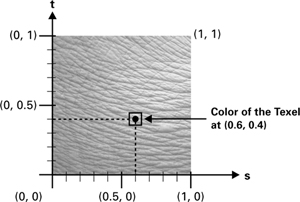
\includegraphics[width=1\linewidth]{fig3_2.jpg}
    \caption{Figure 3-2 Querying a Texture}
    \label{fig:3-2}
\end{figure}

The semantic for the texture coordinate set named \textbf{texCoord} in Example 3-3 is \textbf{TEXCOORD0}, corresponding to the texture coordinate set for texture unit 0. As the name of the sampler parameter \textbf{decal} implies, the intent of this fragment program is to use the fragment's interpolated texture coordinate set to access a texture.

\subsection{3.2.2 Sampling Textures}

The next interesting line of \textbf{C3E3f_texture} accesses the decal texture with the interpolated texture coordinates:

\FloatBarrier
\begin{lstlisting}
   OUT.color = tex2D(decal, texCoord);
\end{lstlisting}
\FloatBarrier

The routine \textbf{tex2D} belongs to the Cg Standard Library. It is a member of a family of routines that access different types of samplers with a specified texture coordinate set and then return a vector result. The result is the sampled data at the location indicated by the texture coordinate set in the sampler object.

In practice, this amounts to a texture lookup. How the texture is sampled and filtered depends on the texture type and texture parameters of the texture object associated with the Cg sampler variable. You can determine the texture properties for a given texture by using OpenGL or Direct3D texture specification commands, depending on your choice of 3D programming interface. Your application is likely to establish this association by using the Cg runtime.

The \textbf{2D} suffix indicates that \textbf{tex2D} must sample a sampler object of type \textbf{sampler2D}. Likewise, the \textbf{texCUBE} routine returns a vector, accepts a sampler of type \textbf{samplerCUBE} for its first argument, and requires a three-component texture coordinate set for its second argument.

Basic fragment profiles (such as \textbf{ps_1_1} and \textbf{fp20}) limit texture-sampling routines, such as \textbf{tex2D} and \textbf{texCUBE}, to the texture coordinate set that corresponds to the sampler's texture unit. To be as simple as possible and support all fragment profiles, the \textbf{C3E3f_texture} example follows this restriction. (See Section 2.3.1 for a brief introduction to profiles.)

Advanced fragment profiles (such as \textbf{ps_2_x}, \textbf{arbfp1}, and \textbf{fp30}) allow a sampler to be sampled using texture coordinate sets from other texture units, or even texture coordinates computed in your Cg program.

\subsection{3.2.3 Sending Texture Coordinates While Sampling a Texture}

The \textbf{C3E2v_varying} vertex program passes a per-vertex position, color, and texture coordinate set to the rasterizer. The \textbf{C3E3f_texture} fragment program ignores the interpolated color, but samples a texture image with the interpolated texture coordinate set. Figure \ref{fig:3-3} shows what happens when you first bind both Cg programs with a texture that contains the image of a gruesome face, and then render our simple triangle with additional per-vertex texture coordinates assigned.

\begin{figure}
    \centering
    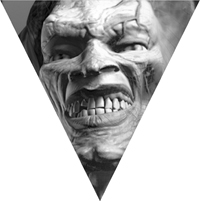
\includegraphics[width=1\linewidth]{fig3_3.jpg}
    \caption{Figure 3-3 Rendering a Textured 2D Triangle with \textbf{C3E2v_varying} and \textbf{C3E3f_texture}}
    \label{fig:3-3}
\end{figure}

\section{3.3 Math Expressions}

So far, all the Cg examples we've presented have done little more than pass along parameters, or use a parameter to sample a texture. Conventional nonprogrammable 3D programming interfaces can accomplish just as much. The point of these examples was to introduce you to Cg and show the structure of simple Cg programs.

More interesting Cg programs perform computations on input parameters by using operators and built-in functions provided by the Cg Standard Library.

\subsection{3.3.1 Operators}

Cg supports the same arithmetic, relational, and other operators provided by C and C++. This means that addition is expressed with a \textbf{+} sign, multiplication with a \textbf{*} symbol, and greater-than-or-equal-to with the \textbf{>=} operator. You have already seen in prior examples that assignment is accomplished with the \textbf{=} sign.

Here are some examples of Cg expressions:

\FloatBarrier
\begin{lstlisting}
float total = 0.333 * (red + green + blue);
total += 0.333 * alpha;
float smaller = (a < b) ? a : b;
float eitherOption = optionA || optionB;
float allTrue = v[0] && v[1] && v[2];
\end{lstlisting}
\FloatBarrier

Cg is different from C and C++ because it provides built-in support for arithmetic operations on vector quantities. You can accomplish this in C++ by writing your own classes that use operator overloading, but vector math operations are a standard part of the language in Cg.

The following operators work on vectors in a component-wise fashion:

\FloatBarrier
\begin{tabular}{ |c|c| } 
\textbf{*} & Multiplication \\
\textbf{/} & Division \\
\textbf{-} & Negation \\
\textbf{+} & Addition \\
\textbf{-} & Subtraction \\
\end{tabular}
\FloatBarrier

When a scalar and a vector are used as operands of one of these component-wise operators, the scalar value is replicated (sometimes called "smeared") into a vector of the matching size.

Here are some examples of vector Cg expressions:

\FloatBarrier
\begin{lstlisting}
float3 modulatedColor = color * float3(0.2, 0.4, 0.5);
modulatedColor *= 0.5;
float3 specular = float3(0.1, 0.0, 0.2);
modulatedColor += specular;
negatedColor = -modulatedColor;
float3 direction = positionA - positionB;
\end{lstlisting}
\FloatBarrier

Table \ref{table:3-2} presents the complete list of operators, along with their precedence, associativity, and usage. Operators marked with a reverse highlight are currently reserved. However, no existing Cg profiles support these reserved operators because current graphics hardware does not support bitwise integer operations.

\begin{table}
\centering
\begin{tabular}{ |c|c|c| } 
 \hline
Operators & Associativity & Usage \\
\hline
\verb|}( ) [ ] -> .| & Left to right & Function call, array reference, structure reference, component selection \\
\verb|! ~ ++ - + - * & (type) sizeof| & Right to left & Unary operators: negation, increment, decrement, positive, negative, indirection, address, cast \\
\verb|* / %| & Left to right & Multiplication, division, remainder \\
\verb|+ -| & Left to right & Addition, subtraction \\
\verb|<< >>| & Left to right & Shift operators \\
\verb|< <= > >=| & Left to right & Relational operators \\
\verb|== !=| & Left to right & Equality, inequality \\
\verb|&| & Left to right & Bitwise AND \\
\verb|^| & Left to right & Bitwise exclusive OR \\
\verb!|! & Left to right & Bitwise OR \\
\verb|&&| & Left to right & Logical AND \\
\verb!||! & Left to right & Logical OR \\
\verb|?| : & Right to left & Conditional expression \\
\verb!= += -= *= /= %= &= ^= |= <<= >>=! & Right to left & Assignment, assignment expressions \\
\verb|,| & Left to right & Comma operator \\
\hline
\end{tabular}

\caption{Table 3-2. Precedence, Associativity, and Usage of Operators}
\label{table:3-2}

\textbf{Notes}
\begin{itemize}
\item Operators are listed top to bottom, from highest to lowest precedence.
\item Operators in the same row have the same precedence.
\item Operators marked with a reverse highlight are currently reserved for future use.
\end{itemize}

\end{table}

\subsection{3.3.2 Profile-Dependent Numeric Data Types}

When you program in C or C++ and declare variables, you pick from a few different-sized integer data types (\textbf{int}, \textbf{long}, \textbf{short}, \textbf{char}) and a couple of different-sized floating-point data types (\textbf{float}, \textbf{double}).

Your CPU provides the hardware support for all these basic data types. However, GPUs do not generally support so many data types—though, as GPUs evolve, they promise to provide more data types. For example, existing GPUs do not support pointer types in vertex or fragment programs.

\subsection*{Representing Continuous Data Types}

Cg provides the \textbf{float}, \textbf{half}, and \textbf{double} floating-point types. Cg's approach to defining these types is similar to C's—the language does not mandate particular precisions. It is understood that \textbf{half} has a range and precision less than or equal to the range and precision of \textbf{float}, and \textbf{float} has a range and precision less than or equal to the range and precision of \textbf{double}.

The \textbf{half} data type does not exist in C or C++. This new data type introduced by Cg holds a half-precision floating-point value (typically 16-bit) that is more efficient in storage and performance than standard-precision floating-point (typically 32-bit) types.

\subsection*{CineFX}

The NVIDIA CineFX GPU architecture supports half-precision values for fragment programs. The \textbf{half} data type is often appropriate for intermediate values in fragment programs, such as colors and normalized vectors. By using \textbf{half} values when possible rather than \textbf{float}, you speed up the performance of your fragment programs.
\hrule

GPUs, by design, provide data types that represent continuous quantities, such as colors and vectors. GPUs do not (currently) support data types that represent inherently discrete quantities, such as alphanumeric characters and bit masks, because GPUs do not typically operate on this kind of data.

Continuous quantities are not limited to integer values. When programming a CPU, programmers typically use floating-point data types to represent continuous values because floating-point types can represent fractional values. Continuous values processed by GPUs, particularly at the fragment level, have been limited to narrow ranges such as [0, 1] or [-1, +1], rather than supporting the expansive range provided by floating-point. For example, colors are often limited to the [0, 1] range, and normalized vectors are, by definition, confined to the [-1, +1] range. These range-limited data types are known as "fixed-point," rather than floating-point.

Although fixed-point data types use limited precision, they can represent continuous quantities. However, they lack the range of floating-point data types, whose encoding is similar to scientific notation. A floating-point value encodes a variable exponent in addition to a mantissa (similar to how numbers are written in scientific notation, such as 2.99 x 108), whereas a fixed-point value assumes a fixed exponent. For example, an unnormalized vector or a sufficiently large texture coordinate may require floating-point for the value to avoid overflowing a given fixed-point range.

Current GPUs handle floating-point equally well when executing vertex and fragment programs. However, earlier programmable GPUs provide floating-point data types only for vertex processing; they offer only fixed-point data types for fragment processing.

Cg must be able to manipulate fixed-point data types to support programmability for GPUs that lack floating-point fragment programmability. This means that certain fragment profiles use fixed-point values. Table 3-3 lists various Cg profiles and describes how they represent various data types. The implication for Cg programmers is that \textbf{float} may not actually mean floating-point in all profiles in all contexts.

\subsection*{Caution}

The \textbf{fp20} and \textbf{ps_1_1} profiles treat variables in fragment coloring as fixed-point values in the range [-1, +1]. By fragment coloring, we mean math operations performed after the texture mapping results. If you want true floating-point data types, use the \textbf{arbfp1}, \textbf{fp30}, or \textbf{vp_2_0} profiles, but be aware these are advanced profiles not supported by older GPUs.
\hrule

\subsection*{CineFX}

The CineFX architecture also supports a special high-performance continuous data type called \textbf{fixed} for fragment programs. The \textbf{fixed} data type has a [-2, +2) range (meaning, ranging from negative 2 to not quite positive 2) for the \textbf{fp30} profile. In other profiles, the \textbf{fixed} data type is synonymous with the smallest continuous data type available. Although the Cg compiler (\textbf{cgc}) and runtime support the \textbf{fixed} data type (and vector versions such as \textbf{fixed3} and \textbf{fixed4}), Microsoft's HLSL compiler (\textbf{fxc}) does not.
\hrule

\begin{table}
\centering
\begin{tabular}{ p{2cm} p{2cm} p{7cm}  } 

Profile Names & Types & Numerics \\
\hline

\multirow{2}{4em}{\textbf{arbfp1} \newline \textbf{arbvp1} \newline \textbf{vs_1_1} \newline \textbf{vs_2_0} \newline \textbf{vp20} \newline \textbf{vp30} } & \textbf{float} \newline \textbf{double} \newline \textbf{half} \newline \textbf{fixed} & Floating-point \\
\cline{2-3}
& \textbf{int} \newline & Floating-point clamped to integers \\
\hline

\textbf{fp20} & \textbf{float} \newline \textbf{double} \newline \textbf{half} \newline \textbf{int} \newline \textbf{fixed} & Floating-point for texture mapping; fixed point with [-1, +1] range for fragment coloring \\
\hline

\textbf{ps_1_1} \newline \textbf{ps_1_2} \newline \textbf{ps_1_3} & \textbf{float} \newline \textbf{double} \newline \textbf{half} \newline \textbf{int} \newline \textbf{fixed} & Floating-point for texture mapping; fixed-point with GPU-dependent range for fragment coloring; range depends on underlying Direct3D capability \\
\hline

\multirow{4}{4em}{\textbf{ps_2_0} \newline \textbf{ps_2_x}} & \textbf{float} \newline \textbf{double} & 24-bit floating-point (minimum)\\
\cline{2-3}
& \textbf{int} & Floating-point clamped to integers \\
\cline{2-3}
& \textbf{half} & 16-bit floating-point (minimum) \\
\cline{2-3}
& \textbf{fixed} & Depends on compiler settings\\
\hline

\multirow{4}{4em}{\textbf{fp30}} & \textbf{float} \newline \textbf{double} & Floating-point \\
\cline{2-3}
& \textbf{int} & Floating-point clamped to integers \\
\cline{2-3}
& \textbf{half} & 16-bit floating-point \\
\cline{2-3}
& \textbf{fixed} & Fixed-point with [-2, 2) range \\
\hline

\end{tabular}

\caption{Table 3-3. Data Types for Various Profiles}
\label{table:3-3}
\end{table}

\subsection{3.3.3 Standard Library Built-In Functions}

The Cg Standard Library contains many built-in functions that simplify GPU programming. In many cases, the functions map to a single native GPU instruction, so they can be very efficient.

These built-in functions are similar to C's Standard Library functions. The Cg Standard Library provides a practical set of trigonometric, exponential, vector, matrix, and texture functions. But there are no Cg Standard Library routines for input/output, string manipulation, or memory allocation, because Cg does not support these operations (though your C or C++ application certainly could).

We already used one Cg Standard Library function, \textbf{tex2D}, in Example 3-3. Refer to Table 3-4 for a select list of other functions that the Cg Standard Library provides. You can find a complete list of Cg Standard Library functions in Appendix E.

\begin{table}
\centering
\begin{tabular}{ p{3cm} p{3cm} p{5cm}  } 

Function Prototype & Profile Usage & Description \\
\hline

\textbf{abs(x)} & All & Absolute value \\
\hline
\textbf{cos(x)} & Vertex, advanced fragment & Cosine of angle in radians \\
\hline
\textbf{cross(v1, v2)} & Vertex, advanced fragment & Cross product of two vectors \\
\hline
\textbf{ddx(a)} \newline \textbf{ddy(a)} & Advanced fragment & Approximate partial derivatives of \textbf{a} with respect to window-space \textbf{x} or \textbf{y} coordinate, respectively \\
\hline
\textbf{determinant(M)} & Vertex, advanced fragment & Determinant of a matrix \\
\hline
\textbf{dot(a, b)} & All, but restricted basic fragment & Dot product of two vectors \\
\hline
\textbf{floor(x)} & Vertex, advanced fragment & Largest integer not greater than \textbf{x} \\
\hline
\textbf{isnan(x)} & Advanced vertex and fragment & True if \textbf{x} is not a number (NaN) \\
\hline
\textbf{lerp(a, b, f)} & All & Linear interpolation between \textbf{a} and \textbf{b} based on \textbf{f} \\
\hline
\textbf{log2(x)} & Vertex, advanced fragment & Base 2 logarithm of \textbf{x} \\
\hline
\textbf{max(a, b)} & All & Maximum of \textbf{a} and \textbf{b} \\
\hline
\textbf{mul(M, N)} \newline \textbf{mul(M, v)} \newline \textbf{mul(v, M)} & Vertex, advanced fragment & 
Matrix-by-matrix multiplication \newline Matrix-by-vector multiplication \newline Vector-by-matrix multiplication \\
\hline
\textbf{pow(x, y)} & Vertex, advanced fragment & Raise \textbf{x} to the power \textbf{y} \\
\hline
\textbf{radians(x)} & Vertex, advanced fragment & Degrees-to-radians conversion \\
\hline
\textbf{reflect(v, n)} & Vertex, advanced fragment & Reflection vector of entering ray \textbf{v} and normal vector \textbf{n} \\
\hline
\textbf{round(x)} & Vertex, advanced fragment & Round \textbf{x} to nearest integer \\
\hline
\textbf{rsqrt(x)} & Vertex, advanced fragment & Reciprocal square root \\
\hline
\textbf{tex2D(sampler, x)} & Fragment, restricted for basic & 2D texture lookup \\
\hline
\textbf{tex3Dproj(sampler, x)} & Fragment, restricted for basic & Projective 3D texture lookup \\
\hline
\textbf{texCUBE(sampler, x)} & Fragment, restricted for basic & Cube-map texture lookup \\
\hline
\end{tabular}

\caption{Table 3-4. Selected Cg Standard Library Functions}
\label{table:3-4}
\end{table}

\subsection*{Function Overloading}

The Cg Standard Library "overloads" most of its routines so that the same routine works for multiple data types. As in C++, function overloading provides multiple implementations for a routine by using a single name and differently typed parameters.

Overloading is very convenient. It means you can use a function, for example \textbf{abs}, with a scalar parameter, a two-component parameter, a three-component parameter, or a four-component parameter. In each case, Cg "calls" the appropriate version of the absolute value function:

\FloatBarrier
\begin{lstlisting}
float4 a4 = float4(0.4, -1.2, 0.3, 0.2);
float2 b2 = float2(-0.3, 0.9);
float4 a4abs = abs(a4);
float2 b2abs = abs(b2);
\end{lstlisting}
\FloatBarrier

The code fragment calls the \textbf{abs} routine twice. In the first instance, \textbf{abs} accepts a four-component vector. In the second instance, \textbf{abs} accepts a two-component vector. The compiler automatically calls the appropriate version of \textbf{abs}, based on the parameters passed to the routine. The extensive use of function overloading in the Cg Standard Library means you do not need to think about what routine to call for a given-size vector or other parameter. Cg automatically picks the appropriate implementation of the routine you name.

Function overloading is not limited to the Cg Standard Library. Additionally, you can write your own internal functions with function overloading.

Function overloading in Cg can even apply to different implementations of the same routine name for different profiles. For example, an advanced vertex profile for a new GPU may have special instructions to compute the trigonometric sine and cosine functions. A basic vertex profile for older GPUs may lack that special instruction. However, you may be able to approximate sine or cosine with a sequence of supported vertex instructions, although with less accuracy. You could write two functions and specify that each require a particular profile.

Cg's support for profile-dependent overloading helps you isolate profile-dependent limitations in your Cg programs to helper functions. The \textit{Cg Toolkit User's Manual: A Developer's Guide to Programmable Graphics} has more information about profile-dependent overloading.

\subsection*{The Cg Standard Library's Efficiency and Precision}

Whenever possible, use the Cg Standard Library to do math or other operations it supports. The Cg Standard Library functions are as efficient and precise as—or more efficient and precise than—similar functions you might write yourself.

For example, the \textbf{dot} function computes the dot product of two vectors. You might write a dot product function yourself, such as this one:

\FloatBarrier
\begin{lstlisting}
float myDot(float3 a, float3 b)
{
  return a[0]*b[0] + a[1]*b[1] + a[2]*b[2];
}
\end{lstlisting}
\FloatBarrier

This is the same math that the \textbf{dot} function implements. However, the \textbf{dot} function maps to a special GPU instruction, so the dot product provided by the Cg Standard Library is very likely to be faster and more accurate than the \textbf{myDot} routine.

\subsection*{Coding Tip}

By using Cg Standard Library functions wherever possible, you guide the Cg compiler to generate the most efficient and precise program for your particular GPU.
\hrule

\subsection{3.3.4 2D Twisting}

In the next example you will put expressions, operators, and the Cg Standard Library to work. This example demonstrates how to twist 2D geometry. The farther a vertex is from the center of the window, the more the vertex program rotates the vertex around the center of the window.

The \textbf{C3E4v_twist} program shown in Example 3-4 demonstrates scalar-by-vector multiplication, scalar addition and multiplication, scalar negation, the \textbf{length} Standard Library routine, and the \textbf{sincos} Standard Library routine.

\FloatBarrier
\begin{lstlisting}[caption=Example 3-4. The \textbf{C3E4v_twist} Vertex Program]
struct C3E4_Output {
  float4 position : POSITION;
  float4 color    : COLOR;
};

C3E4_Output C3E4v_twist(float2 position : POSITION,
                        float4 color    : COLOR,

                        uniform float twisting)
{
  C3E4_Output OUT;
  float angle = twisting * length(position);
  float cosLength, sinLength;
  sincos(angle, sinLength, cosLength);
  OUT.position[0] = cosLength * position[0] +
                   -sinLength * position[1];
  OUT.position[1] = sinLength * position[0] +
                    cosLength * position[1];
  OUT.position[2] = 0;
  OUT.position[3] = 1;
  OUT.color = color;
  return OUT;
}
\end{lstlisting}
\FloatBarrier

The \textbf{C3E4v_twist} program inputs the vertex \textbf{position} and \textbf{color} as varying parameters and a uniform scalar \textbf{twisting} scale factor. Figure \ref{fig:3-4} shows the example with various amounts of twisting.

\begin{figure}
    \centering
    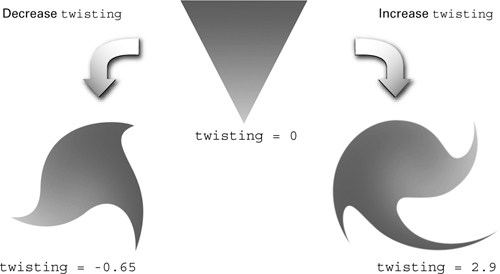
\includegraphics[width=1\linewidth]{fig3_4.jpg}
    \caption{Figure 3-4 \textbf{C3E4v_twist} Results with Different Parameter Settings}
    \label{fig:3-4}
\end{figure}

\subsection*{The length and sincos Standard Library Routines}

The \textbf{length} routine has an overloaded prototype, where \textit{SCALAR} is any scalar data type and \textit{VECTOR} is a vector of the same scalar data type as \textit{SCALAR} with one, two, three, or four components:

\FloatBarrier
\begin{lstlisting}
SCALAR length(VECTOR x);
\end{lstlisting}
\FloatBarrier

The Cg Standard Library routine \textbf{length} returns the scalar length of its single input parameter:

\FloatBarrier
\begin{lstlisting}
  float angle = twisting * length(position);
\end{lstlisting}
\FloatBarrier

The program computes an angle in radians that is the \textbf{twisting} parameter times the length of the input position. Then the \textbf{sincos} Standard Library routine computes the sine and cosine of this angle.

The \textbf{sincos} routine has the following overloaded prototype, where \textit{SCALAR} is any scalar data type:

\FloatBarrier
\begin{lstlisting}
void sincos(SCALAR angle, out SCALAR s, out SCALAR c);
\end{lstlisting}
\FloatBarrier

When \textbf{sincos} returns, Cg updates the calling parameters \textbf{s} and \textbf{c} with the sine and cosine, respectively, of the \textbf{angle} parameter (assumed to be in radians).

\subsection*{Advanced: Call-by-Result Parameter Passing}

An \textbf{out} qualifier indicates that when the routine returns, Cg must assign the final value of a formal parameter qualified by \textbf{out} to its corresponding caller parameter. Initially, the value of an \textbf{out} parameter is undefined. This convention is known as \textit{call-by-result} (or \textit{copy-out}) parameter passing.

C has no similar parameter-passing convention. C++ allows a reference parameter to function (indicated by \textbf{\&} prefixed to formal parameters), but this is a \textit{call-by-reference} parameter-passing convention, not Cg's call-by-result convention.

Cg also provides the \textbf{in} and \textbf{inout} keywords. The \textbf{in} type qualifier indicates that Cg passes the parameter by value, effectively \textit{call-by-value}. The calling routine's parameter value initializes the corresponding formal parameter of the routine called. When a routine with \textbf{in}-qualified parameters returns, Cg discards the values of these parameters unless the parameter is also \textbf{out}-qualified.

C uses the copy-by-value parameter-passing convention for all parameters. C++ uses copy-by-value for all parameters, except those passed by reference.

The \textbf{inout} type qualifier (or the \textbf{in} and \textbf{out} type qualifiers that are specified for a single parameter) combine call-by-value with call-by-result (otherwise known as \textit{call-by-value-result} or \textit{copy-in-copy-out}).

The \textbf{in} qualifier is optional because if you do not specify an \textbf{in}, \textbf{out}, or \textbf{inout} qualifier, the \textbf{in} qualifier is assumed.

You can use \textbf{out} and \textbf{inout} parameters and still return a conventional return value.

\subsection*{Rotating Vertices}

Once the program has computed the sine and cosine of the angle of rotation for the vertex, it applies a rotation transformation. Equation 3-1 expresses 2D rotation.

\FloatBarrier
\begin{equationcaption}
\centering
$
\begin{bmatrix}
x' \\
y' \\
\end{bmatrix}
= 
\begin{bmatrix}
cos \theta & -sin \theta \\
sin \theta & cos \theta \\
\end{bmatrix}
\begin{bmatrix}
x \\
y \\
\end{bmatrix}
$
\caption{Equation 3-1 2D Rotation}
\end{equationcaption}
\FloatBarrier

The following code fragment implements this equation. In Chapter 4, you will learn how to express this type of matrix math more succinctly and efficiently, but for now we'll implement the math the straightforward way:

\FloatBarrier
\begin{lstlisting}
   OUT.position[0] = cosLength * position[0] +
                    -sinLength * position[1];
   OUT.position[1] = sinLength * position[0] +
                     cosLength * position[1];
\end{lstlisting}
\FloatBarrier

\subsection*{The Importance of Tessellation for Vertex Programs}

The \textbf{C3E4v_twist} program works by rotating vertices around the center of the image. As the magnitude of the twist rotation increases, an object may require more vertices—thus higher tessellation—to reproduce the twisting effect reasonably.

Generally, when a vertex program involves nonlinear computations, such as the trigonometric functions in this example, sufficient tessellation is required for acceptable results. This is because the values of the vertices are interpolated linearly by the rasterizer as it creates fragments. If there is insufficient tessellation, the vertex program may reveal the tessellated nature of the underlying geometry. Figure \ref{fig:3-5} shows how increasing the amount of tessellation improves the twisted appearance of the \textbf{C3E4v_twist} example.

\begin{figure}
    \centering
    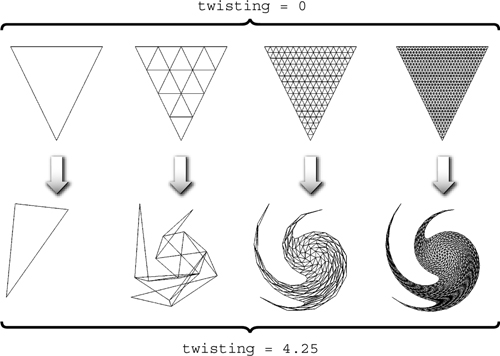
\includegraphics[width=1\linewidth]{fig3_5.jpg}
    \caption{Figure 3-5 Improving the Fidelity of \textbf{C3E4v_twist} by Increasing Tessellation}
    \label{fig:3-5}
\end{figure}

\subsection{3.3.5 Double Vision}

Now we demonstrate how to combine a vertex program and a fragment program to achieve a textured "double vision" effect. The idea is to sample the same texture twice, based on slightly shifted texture coordinates, and then blend the samples equally.

The \textbf{C3E5v_twoTextures} vertex program shown in Example 3-5 shifts a single texture coordinate position twice, using two distinct offsets to generate two slightly separated texture coordinate sets. The fragment program then accesses a texture image at the two offset locations and equally blends the two texture results. Figure \ref{fig:3-6} shows the rendering results and the required inputs.

\FloatBarrier
\begin{lstlisting}[caption=Example 3-5. The \textbf{C3E5v_twoTextures} Vertex Program]
void C3E5v_twoTextures(float2 position : POSITION,
                       float2 texCoord : TEXCOORD0,

                   out float4 oPosition     : POSITION,
                   out float2 leftTexCoord  : TEXCOORD0,
                   out float2 rightTexCoord : TEXCOORD1,

               uniform float2 leftSeparation,
               uniform float2 rightSeparation)
{
  oPosition     = float4(position, 0, 1);
  leftTexCoord  = texCoord + leftSeparation;
  rightTexCoord = texCoord + rightSeparation;
}
\end{lstlisting}
\FloatBarrier

\subsection*{The Double Vision Vertex Program}

The \textbf{C3E5v_twoTextures} program in Example 3-5 passes through the vertex position. The program outputs the single input texture coordinate twice, once shifted by the \textbf{leftSeparation} uniform parameter and then shifted by the \textbf{rightSeparation} uniform parameter.

\FloatBarrier
\begin{lstlisting}
   oPosition     = float4(position, 0, 1);
   leftTexCoord  = texCoord + leftSeparation;
   rightTexCoord = texCoord + rightSeparation;
\end{lstlisting}
\FloatBarrier

\begin{figure}
    \centering
    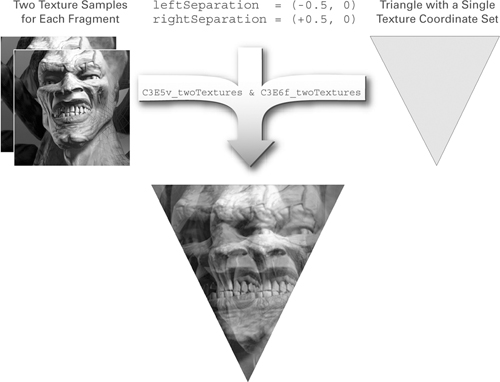
\includegraphics[width=1\linewidth]{fig3_6.jpg}
    \caption{Figure 3-6 Creating a Double Vision Effect with \textbf{C3E5v_twoTextures} and \textbf{C3E5f_twoTextures}}
    \label{fig:3-6}
\end{figure}

\subsection*{Out Parameters vs. Output Structures}

The \textbf{C3E5v_twoTextures} example also shows a different approach to outputting parameters. Rather than return an output structure, as all our previous examples have done, the \textbf{C3E5v_twoTextures} example returns nothing; the function's return type is \textbf{void}. Instead, \textbf{out} parameters with associated semantics, which are part of the entry function's prototype, indicate which parameters are output parameters. The choice of using \textbf{out} parameters or an output return structure to output parameters from an entry function is up to you. There is no functional difference between the two approaches. You can even mix them.

The remainder of this book uses the \textbf{out} parameter approach, because it avoids having to specify output structures. We add an "\textbf{o}" prefix for \textbf{out} parameters to distinguish input and output parameters that would otherwise have the same name—for example, the \textbf{position} and \textbf{oPosition} parameters.

\FloatBarrier
\begin{lstlisting}[caption=Example 3-6. The \textbf{C3E6f_twoTextures} Fragment Program]
void C3E6f_twoTextures(float2 leftTexCoord  : TEXCOORD0,
                       float2 rightTexCoord : TEXCOORD1,

                   out float4 color : COLOR,

               uniform sampler2D decal)
{
  float4 leftColor  = tex2D(decal, leftTexCoord);
  float4 rightColor = tex2D(decal, rightTexCoord);
  color = lerp(leftColor, rightColor, 0.5);
}
\end{lstlisting}
\FloatBarrier

In Example 3-5 and subsequent examples, we also line up and group the parameters to the entry function as input, output, and uniform parameters. This style takes extra work to format code, but we use it in this book to make the examples easier to read, particularly when the examples have many parameters.

\subsection*{The Double Vision Fragment Program for Advanced Fragment Profiles}

The \textbf{C3E6f_twoTextures} fragment program in Example 3-6 takes the two shifted and interpolated texture coordinate sets computed by \textbf{C3E5v_twoTextures} and uses them to sample the same texture image twice, as shown in Figure \ref{fig:3-6}.

\FloatBarrier
\begin{lstlisting}   
   float4 leftColor  = tex2D(decal, leftTexCoord);
   float4 rightColor = tex2D(decal, rightTexCoord);
\end{lstlisting}
\FloatBarrier

Then the program computes the average of the two color samples:

\FloatBarrier
\begin{lstlisting}
  color = lerp(leftColor, rightColor, 0.5);
\end{lstlisting}
\FloatBarrier

The \textbf{lerp} routine computes a weighted linear interpolation of two same-sized vectors. The mnemonic \textit{lerp} stands for "linear interpolation." The routine has an overloaded prototype in which \textit{VECTOR} is a vector with one, two, three, or four components and \textit{TYPE} is a scalar or vector with the same number of components and element types as \textit{VECTOR}:

\FloatBarrier
\begin{lstlisting}
VECTOR lerp(VECTOR a, VECTOR b, TYPE weight);
\end{lstlisting}
\FloatBarrier

The lerp routine computes:

\FloatBarrier
$
result = (1 - weight) * a + weight * b
$
\FloatBarrier

A \textit{weight} of 0.5 gives a uniform average. There is no requirement that the weight be within the 0 to 1 range.

Unfortunately, the \textbf{C3E6f_twoTextures} fragment program will not compile with basic fragment profiles such as \textbf{fp20} and \textbf{ps_1_1} (you will learn why shortly). It compiles fine, however, with advanced fragment profiles, such as \textbf{fp30} and \textbf{ps_2_0}.

\subsection*{The Double Vision Fragment Program for Basic Fragment Profiles}

The \textbf{C3E6f_twoTextures} example uses two texture coordinate sets, 0 and 1, to access texture unit 0. Because of this, the program does not compile with basic fragment program profiles. Such profiles can use only a given texture coordinate set with the set's corresponding texture unit due to limitations in third-generation and earlier GPUs.

You can alter the \textbf{C3E6f_twoTextures} program slightly so that it works with basic and advanced fragment profiles. The \textbf{C3E7f_twoTextures} version in Example 3-7 contains the necessary alterations.

\FloatBarrier
\begin{lstlisting}[caption=Example 3-7. The \textbf{C3E7f_twoTextures} Fragment Program]
void C3E7f_twoTextures(float2 leftTexCoord : TEXCOORD0,
                      float2 rightTexCoord : TEXCOORD1,

                  out float4 color : COLOR,

              uniform sampler2D decal0,
              uniform sampler2D decal1)
{
  float4 leftColor  = tex2D(decal0, leftTexCoord);
  float4 rightColor = tex2D(decal1, rightTexCoord);
  color = lerp(leftColor, rightColor, 0.5);
}
\end{lstlisting}
\FloatBarrier

The modified program requires two texture units:

\FloatBarrier
\begin{lstlisting}                  
                  uniform sampler2D decal0,
                  uniform sampler2D decal1
\end{lstlisting}
\FloatBarrier

So that the two texture units sample the same texture image, the \textbf{C3E7f_twoTextures} fragment program requires the application to bind the same texture for two separate texture units. The original \textbf{C3E6f_twoTextures} program did not require the application to bind the texture twice.

When the program samples the two textures, it samples each texture unit with its corresponding texture coordinate set, as required by basic fragment program profiles:

\FloatBarrier
\begin{lstlisting} 
  float4 leftColor  = tex2D(decal0, leftTexCoord);
  float4 rightColor = tex2D(decal1, rightTexCoord);
\end{lstlisting}
\FloatBarrier

The performance of these two approaches is comparable. This example demonstrates that \textit{simpler} Cg programs—those that are not too complicated—can often be written with a little extra care to run on older GPUs, which support basic vertex and fragment profiles, as well as on recent GPUs, which support advanced profiles.

\section{3.4 Exercises}

\begin{enumerate}
\item \textbf{Answer this:} Beyond mere convenience, why do you suppose the \textbf{sincos} Standard Library routine returns both the sine and the cosine of an angle? \textit{Hint:} Think trigonometric identities.
\item \textbf{Answer this:} Explain in your own words why the increased tessellation shown in Figure 3-5 is required for the twisted triangle to look good.
\item \textbf{Try this yourself:} Modify the \textbf{C3E4v_twist} example so that the twisting centers on some arbitrary 2D point specified as a \textbf{uniform float2} parameter, rather than on the origin (0, 0).
\item \textbf{Try this yourself:} Modify the \textbf{C3E5v_twoTextures} and \textbf{C3E7f_twoTextures} programs to provide "quadruple vision." Make sure your new program works on both basic and advanced profiles. Assume that your GPU supports four texture units.
\item \textbf{Try this yourself:} Modify the \textbf{C3E5v_twoTextures} example to return an output structure rather than use \textbf{out} parameters. Also, modify an earlier example, such as \textbf{C3E4v_twist}, to use \textbf{out} parameters rather than return an output structure. Which approach do you prefer?
\end{enumerate}

\section{3.5 Further Reading}

You can learn more about 2x2 matrices, such as the rotation matrix in the twist example, in \textit{The Geometry Toolbox for Graphics and Modeling} (A. K. Peters, 1998), by Gerald Farin and Dianne Hansford.

\end{document}